\documentclass[12pt]{article}

\usepackage[a4paper, margin=1in]{geometry}

\usepackage{listings}
\usepackage{color}
\usepackage{float}
\usepackage{graphicx}
\usepackage{subcaption}

\definecolor{codegreen}{rgb}{0,0.6,0}
\definecolor{codegray}{rgb}{0.5,0.5,0.5}
\definecolor{codepurple}{rgb}{0.58,0,0.82}
\definecolor{backcolour}{rgb}{0.95,0.95,0.92}

\lstdefinestyle{mystyle}{
  backgroundcolor=\color{backcolour},
  commentstyle=\color{codegreen},
  keywordstyle=\color{magenta},
  numberstyle=\tiny\color{codegray},
  stringstyle=\color{codepurple},
  basicstyle=\ttfamily,
  breakatwhitespace=false,
  breaklines=true,
  captionpos=b,
  keepspaces=true,
  numbers=left,
  numbersep=5pt,
  showspaces=false,
  showstringspaces=false,
  showtabs=false,
  tabsize=2
}

\lstset{style=mystyle}

\setlength\parindent{0pt}
\setlength\parskip{1em}

\title{Lab 10 - Kuwahara}
\author{\textsc{Nguyen} Duc Tung}
\date{}

\begin{document}

\maketitle

This labwork is the longest one with many of the computation steps.
\\\\
The first step is to calculate the HSV color space of all pixels, cause we need the Value for doing the Kuhawara filter
\\\\
Then I wrote a kernel processes each individual pixel. The kernel handle 4 windows surrounding the pixel as follows:

\begin{enumerate}
  \item Find the 2 pivots of a window (1 top left, 1 botton right)
  \item Calculate the standard deviation
  \item Find the window with minimum standard deviation
  \item Compute the mean RGB value of the selected window, and assign it as the new value for the pixel
\end{enumerate}

And following is the result:

\begin{itemize}
  \item Me at the Louvre Museum
  \\\\
  Image size: 1280x960, window size: 5, time elassed: 79.2 ms

  \begin{figure}[H]
    \centering
    \begin{subfigure}{.45\textwidth}
      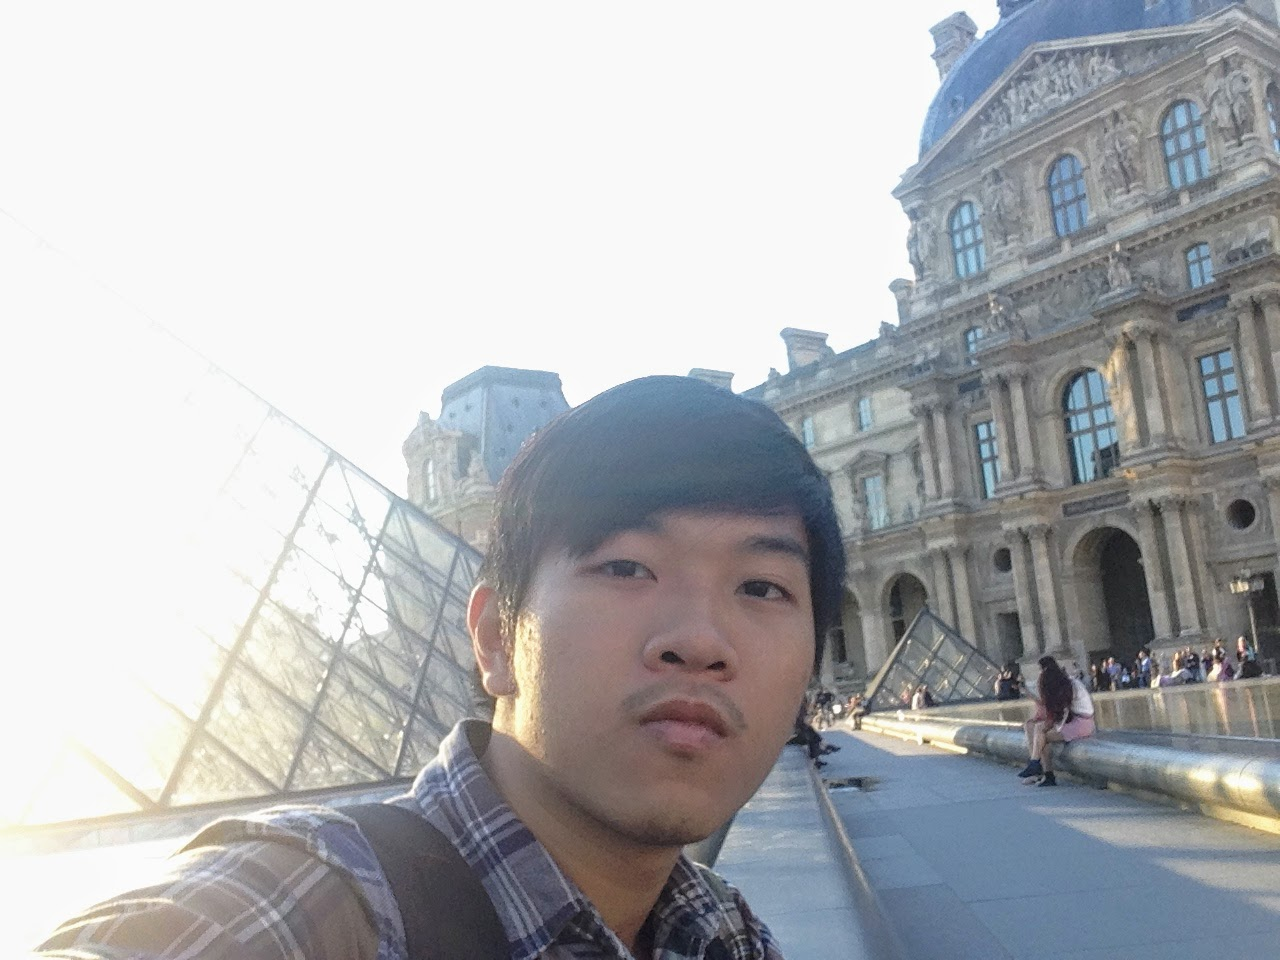
\includegraphics[width=\linewidth]{./img/1_in.jpg}
      \caption{Original image}
    \end{subfigure}
    \hspace{1cm}
    \begin{subfigure}{.45\textwidth}
      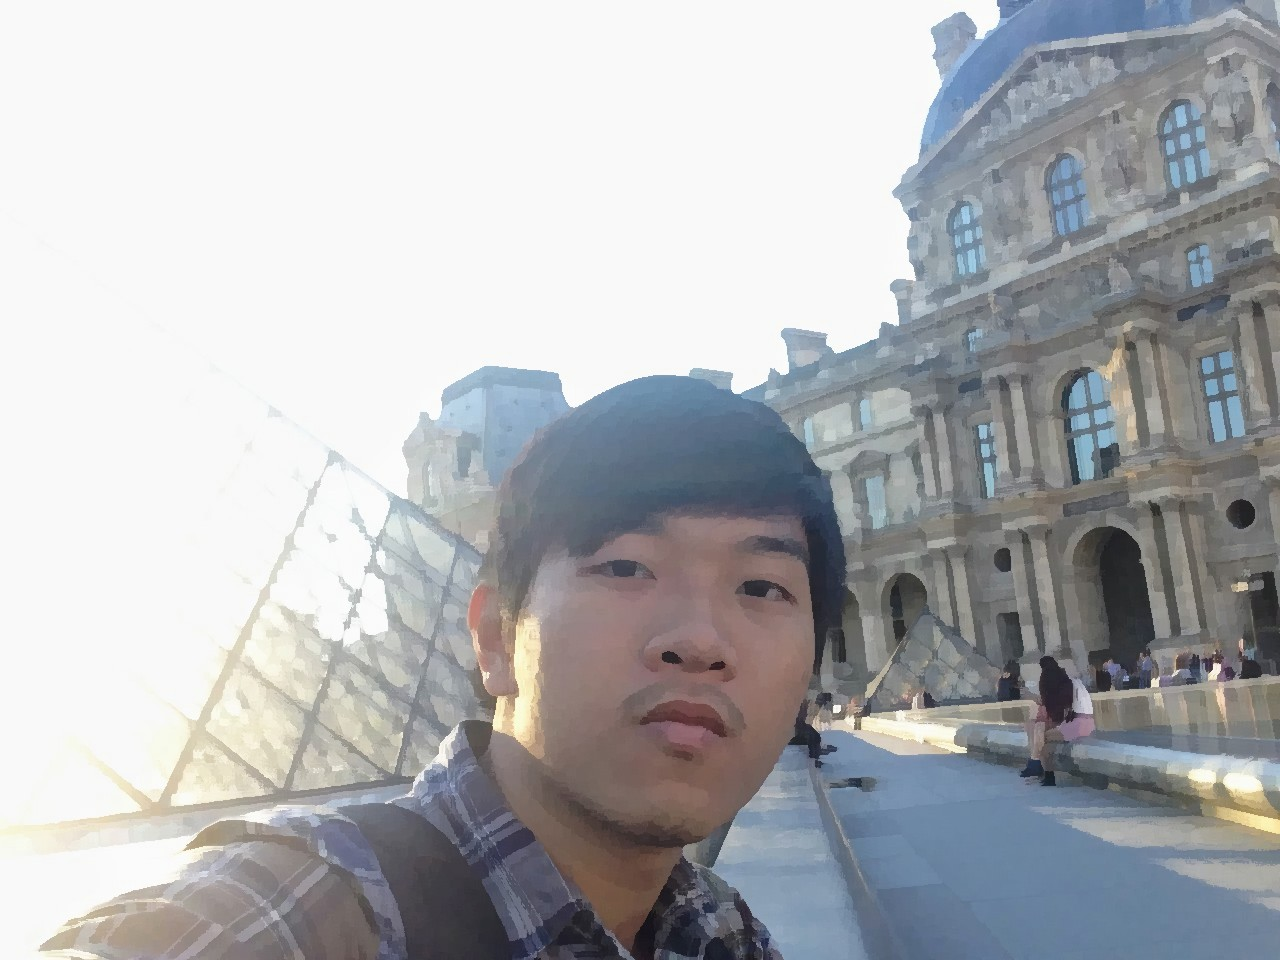
\includegraphics[width=\linewidth]{./img/1_out.jpg}
      \caption{Art}
    \end{subfigure}
  \end{figure}

  \item And my favorite dog breed: Golden Retriever
  \\\\
  Image size: 1600x1200, window size: 15, time elassed: 985.8 ms

  \begin{figure}[H]
    \centering
    \begin{subfigure}{.45\textwidth}
      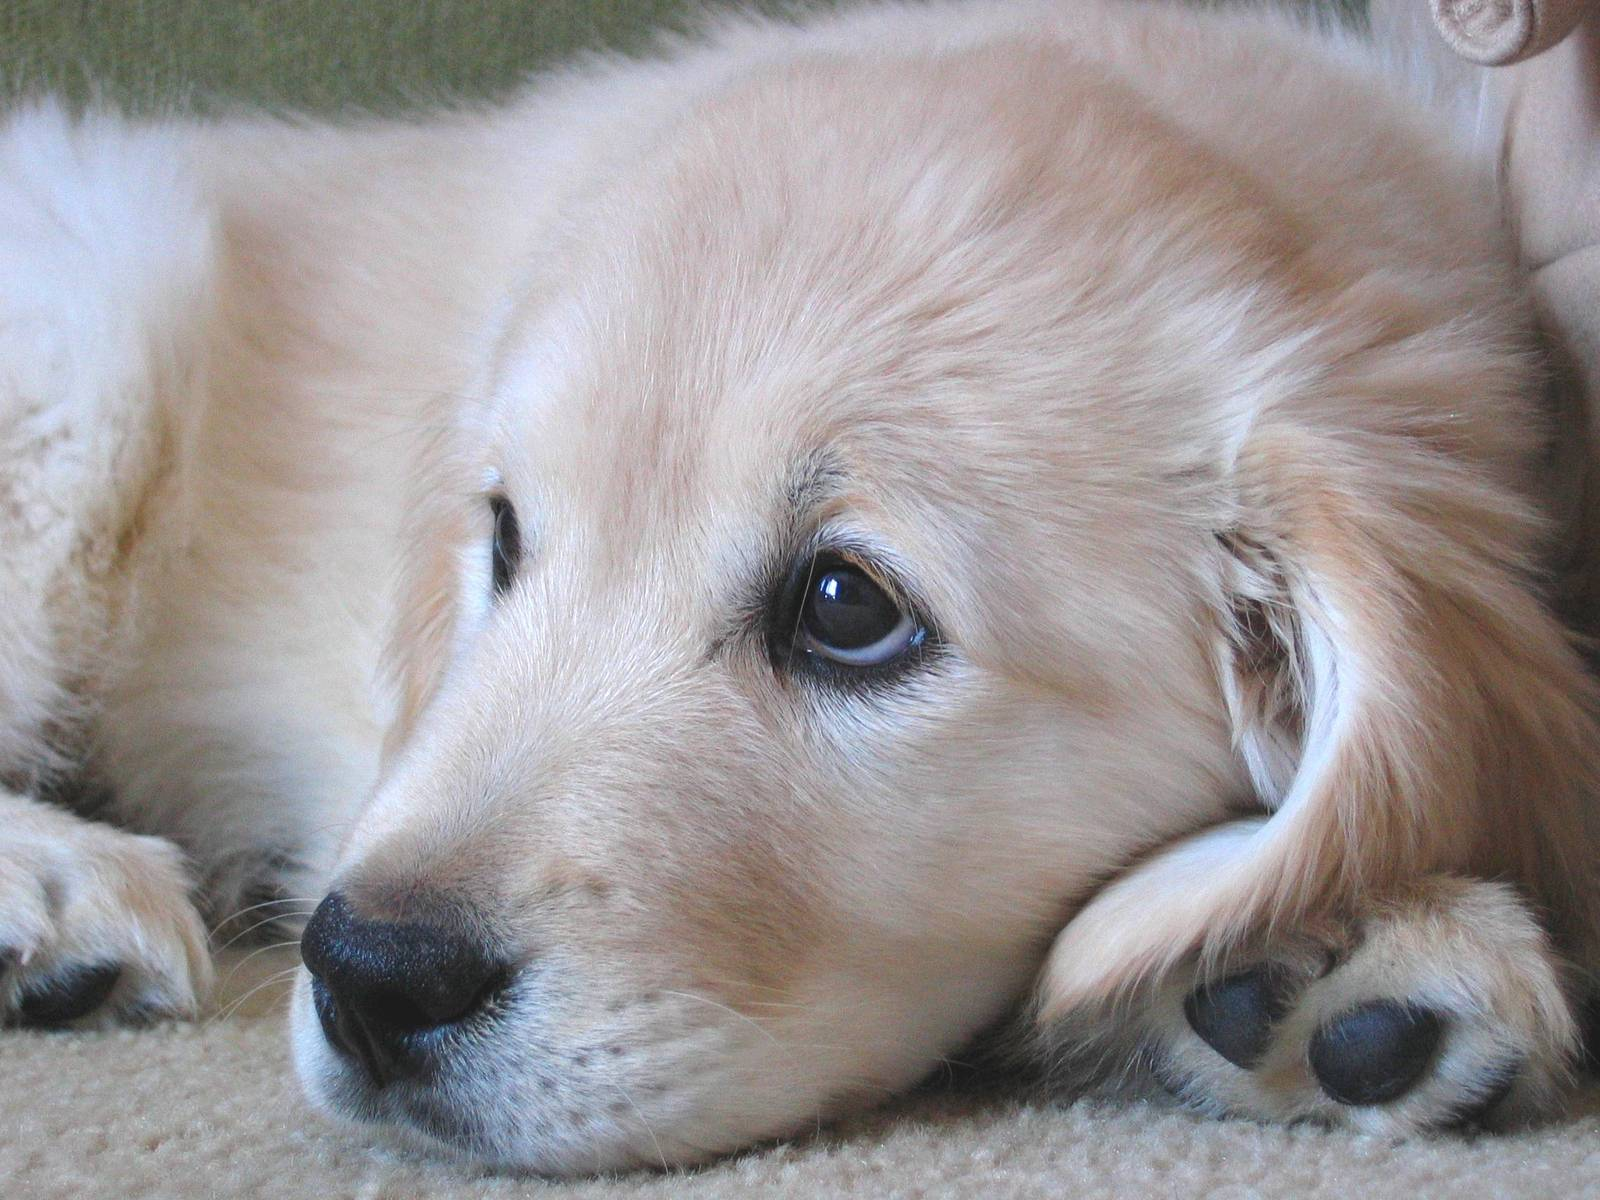
\includegraphics[width=\linewidth]{./img/2_in.jpg}
      \caption{Original image}
    \end{subfigure}
    \hspace{1cm}
    \begin{subfigure}{.45\textwidth}
      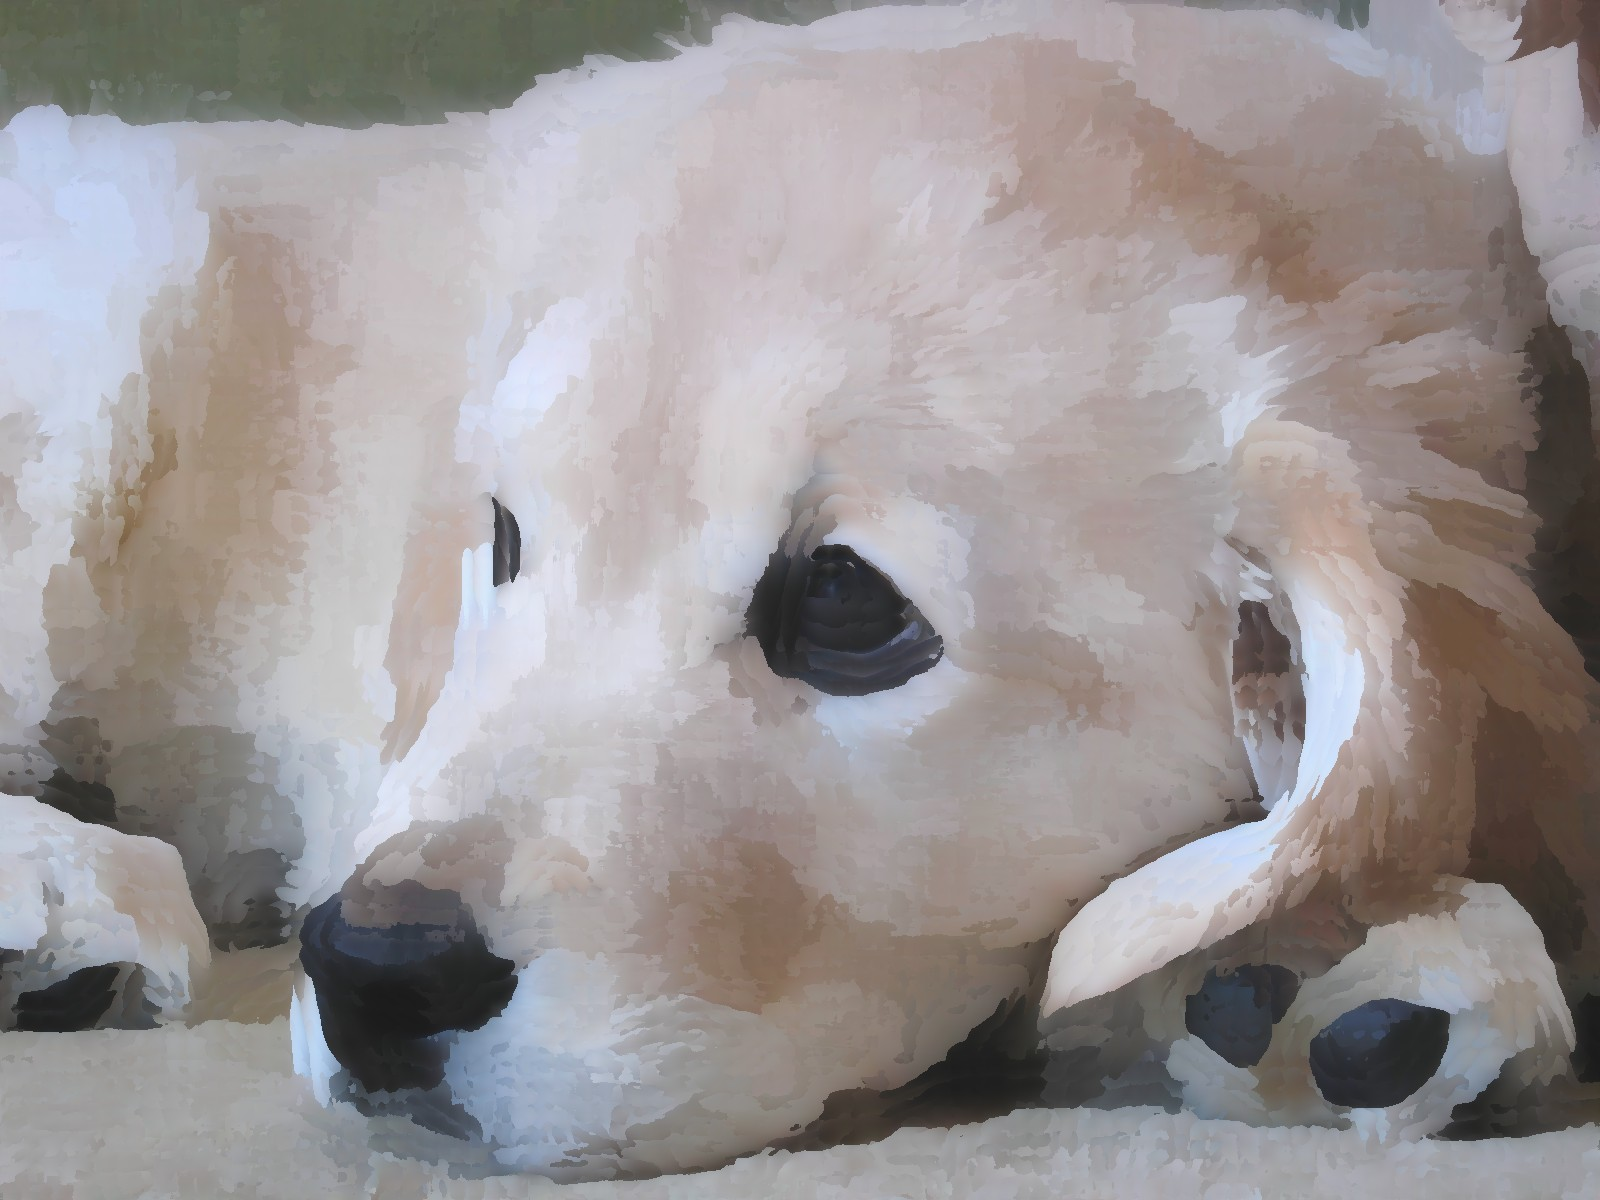
\includegraphics[width=\linewidth]{./img/2_out.jpg}
      \caption{Art}
    \end{subfigure}
  \end{figure}
\end{itemize}

I have some ideas to optimize this implementation but I cannot finished it yet before today. One of the most crucial one is to process all the windows beforehand (calculate the standard deviation, the mean RGB value). Because in this approach, each typical window will be processed at least 4 times for different 4 pixels, which is very computational expensive and redundant.
\\\\
Other than that, there should be a lot of small tweaks for optimizing the kernel. I will try to enhance after the submit.
\\\\
I had fun with this anyway! :D

\end{document}
